\subsection{Oblivious transfer}

Sender $S$ holds $x_1, \ldots, x_n$. Receiver $R$ wants $x_c$, such that $S$
learns nothing of $c$, $R$ learns nothing of $x_{c'} with c' \neq c$.


\subsubsection{2-1 OT from ElGamal}


Idea: $R$ prepares two public keys, $y_0, y_1$, such that it knows the private
key of only $y_c$. Then $S$ can publish both ciphertexts $c_1, c_2$, and $R$
will be able to decrypt only $c_c$ to $x_c$.

\begin{algorithm}
		\caption{2-1 OT using ElGamal}

		\begin{multicols}{2}
				\begin{algorithmic}[0]
						\State \textbf{S}
						\State $r \rgets \mathbb{Z}_q$
						\State $t \coloneqq g^{r} \rightarrow$
						\State
						\State
						\State
						\State
						\If{$t \neq y_0 \cdot y_1$}
						\State \textbf{Halt}
						\EndIf
						\State $(R_0, C_0) \coloneqq Enc(y_0, x_0)$
						\State $(R_1, C_1) \coloneqq Enc(y_1, x_1)$
						\State $\xrightarrow{(R_0, C_0, R_1, C_1)}$
				\end{algorithmic}

				\columnbreak

				\begin{algorithmic}[0]
						\State \textbf{R}
						\State
						\State
						\State $x_c \rgets \mathbb{Z}_q$
						\State $y_c \coloneqq g^{x_c}$
						\State $y_{c'} \coloneqq \frac{t}{y_c}$
						\State $\xleftarrow{y_0, y_1}$
						\State
						\State
						\State
						\State
						\State
						\State \textbf{Return} $Dec(x_c, R_c, C_c)$
				\end{algorithmic}
		\end{multicols}
\end{algorithm}

Security for $S$ based on DL (so $R$ cannot know DL of both $y_0$ and $y_1$)
and security of ElGamal. Security for $R$ unconditional, as it only sends two
identically distributed values.

\section{Secure two-party computation (2PC)}

Goal: Evaluate $f(x, y)$ between parties $A$ and $B$, with $A$ holding $x$, $B$
holding $y$. One of them ($B$) should learn $f(x, y)$, and neither should learn
more of the other's input than $f(x, y)$ itself implies.

\subsection{Toy example using OT}

If domain of $y \in Y$ is small, $A$ prepares $s_y \coloneqq f(x, y) \forall y
\in Y$, and sends $\{s_y\}$ via $1-of-|Y|$ OT to B. $B$ selects output $y$, and
will thus learn $s_y = f(x, y)$ directly.

Issue in general: With $m$-bit input of $B$, the OT would have $2^m$ options.

\subsection{Towards Yao's garbled circuits construction}

Assume asymmetric encryption scheme which allows to check whether a key is the
correct key for a giphen ciphertext. $Dec(k, c)$ returns $\bot$ if $c$ was not
produced as $Enc(k, m)$ for some message $m$.

Can be implemented as e.g. authenticated encryption, or by appending a magic
bitstring to messages before encrypting them, which can be checked for after
decryption.

\subsubsection{Encrypt function table of $f$}

\begin{enumerate}
		\item Represent every $x \in X, y \in Y$ with a random key $k_x, k_y$ respectively.
		\item For $x \in X, y \in Y$ compute $f(x, y)$ and encrypt it in Table
				$T$ at position $T_{x, y}$: $T_{x, y} \coloneqq Enc(k_x \cdot
				k_y, f(x, y))$
		\item Transfer key $k_y$ (of B's input $y$) to $B$, send $k_x$ to B
		\item $B$ tries to decrypt all entries, and succeeds in $f(x, y)$
\end{enumerate}

\begin{algorithm}
		\caption{Encrypted function table of $f$}

		\begin{multicols}{2}
				\begin{algorithmic}[0]
						\State \textbf{A(x)}
						\State $k_x \rgets \{0, 1\}^\lambda \forall x \in X$
						\State $k_y \rgets \{0, 1\}^\lambda \forall x \in X$
						\State $t_{x, y} \coloneqq Enc(k_x \cdot k_y, f(x, y)) \forall x, y$
						\State $T$ random permutation of $t_{x, y}$
						\State $\xrightarrow{T}$
						\State $\xrightarrow{k_{x} \forall x}$
						\State Send $k_y$ to $B$ via $|Y|-1$ OT.
				\end{algorithmic}

				\columnbreak

				\begin{algorithmic}[0]
						\State \textbf{B(y)}
						\State
						\State
						\State
						\State
						\State
						\State
						\State
						\State Receive $k_y$ via $|Y|-1$ OT
						\State Try to decrypt every entry $t_{x, y}$ using every possible key $k_y \cdot k_x \forall x \in X$
						\State Return entry which decrypted
				\end{algorithmic}
		\end{multicols}
\end{algorithm}

\paragraph{Cost}

\begin{itemize}
		\item $m-1$ OT takes $m$ public-key operations
		\item $B$ must try to decrypt all $|X| \cdot |Y|$ rows in $T$
		\item Both can be improved
		\item $A$ sends $T$ of size $O(|X| \cdot |Y| \cdot l)$ bits to $B$,
				cannot be easily improved
\end{itemize}

\subsection{Yao's garbled circuit protocol}

Suppose $f(x, y)$ is given as a logical circuit $C$. Encrypt garbled function
table of each gate in $C$:

\begin{itemize}
		\item Assume gate $G$ has input wires $i, j$, output wire $t$
		\item Represent values on wires with tokens for $Enc$: $k^0_i, k^1_i$
				for input wire $w_i$. $k^0_j, k^1_j$ for input wire $w_j$.
				$k^0_t, k^1_t$ for output wire $w_t$.
		\item For each combination of inputs, encrypt corresponding output key
				with the input tokens:
				\begin{itemize}
						\item $Enc(k^0_i \cdot k^0_j, k^{G(0, 0)}_t)$
						\item $Enc(k^0_i \cdot k^1_j, k^{G(0, 1)}_t)$
						\item $Enc(k^1_i \cdot k^0_j, k^{G(1, 0)}_t)$
						\item $Enc(k^1_i \cdot k^0_j, k^{G(1, 1)}_t)$
				\end{itemize}
		\item Evaluator obtains one key for each wire, with this one it moves
				on to next gate
\end{itemize}

\subsubsection{Generate gabled circuit}

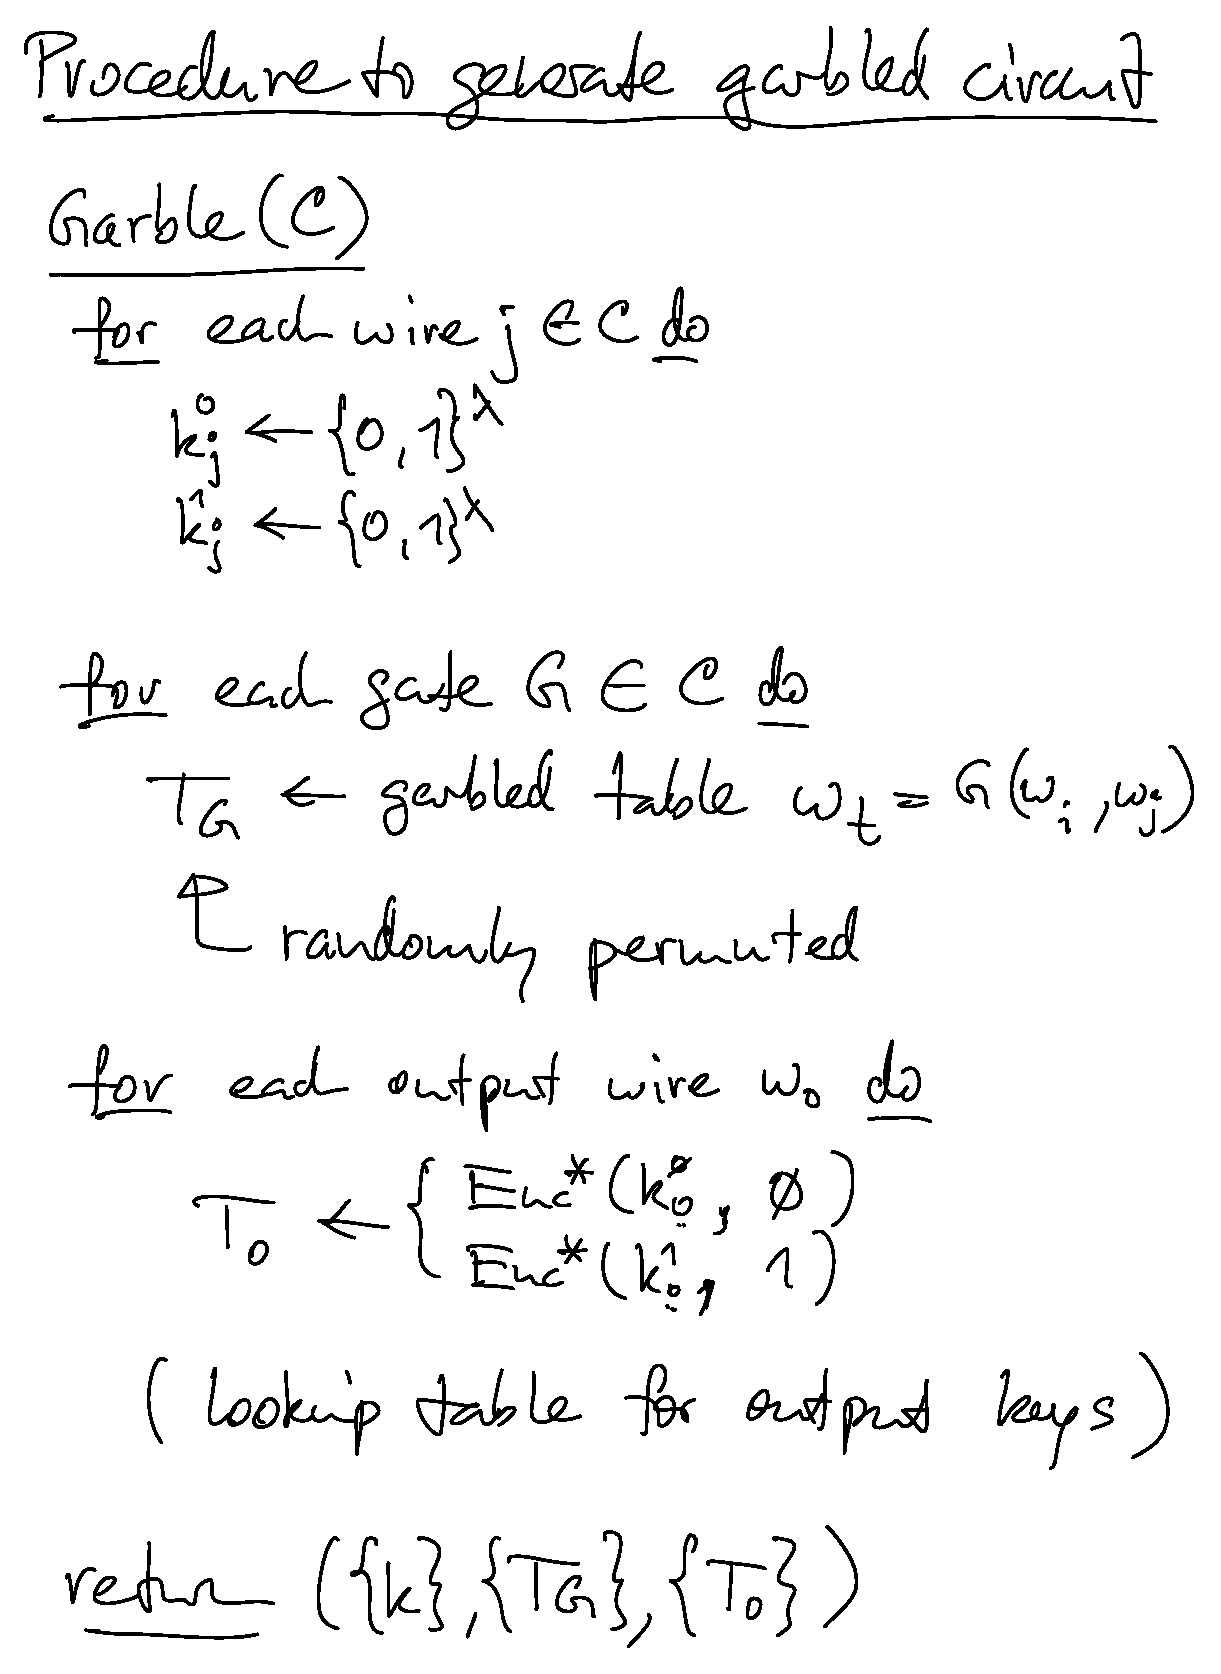
\includegraphics[width=0.7\textwidth]{8_garble}

\subsubsection{Evaluate garbled circuit}

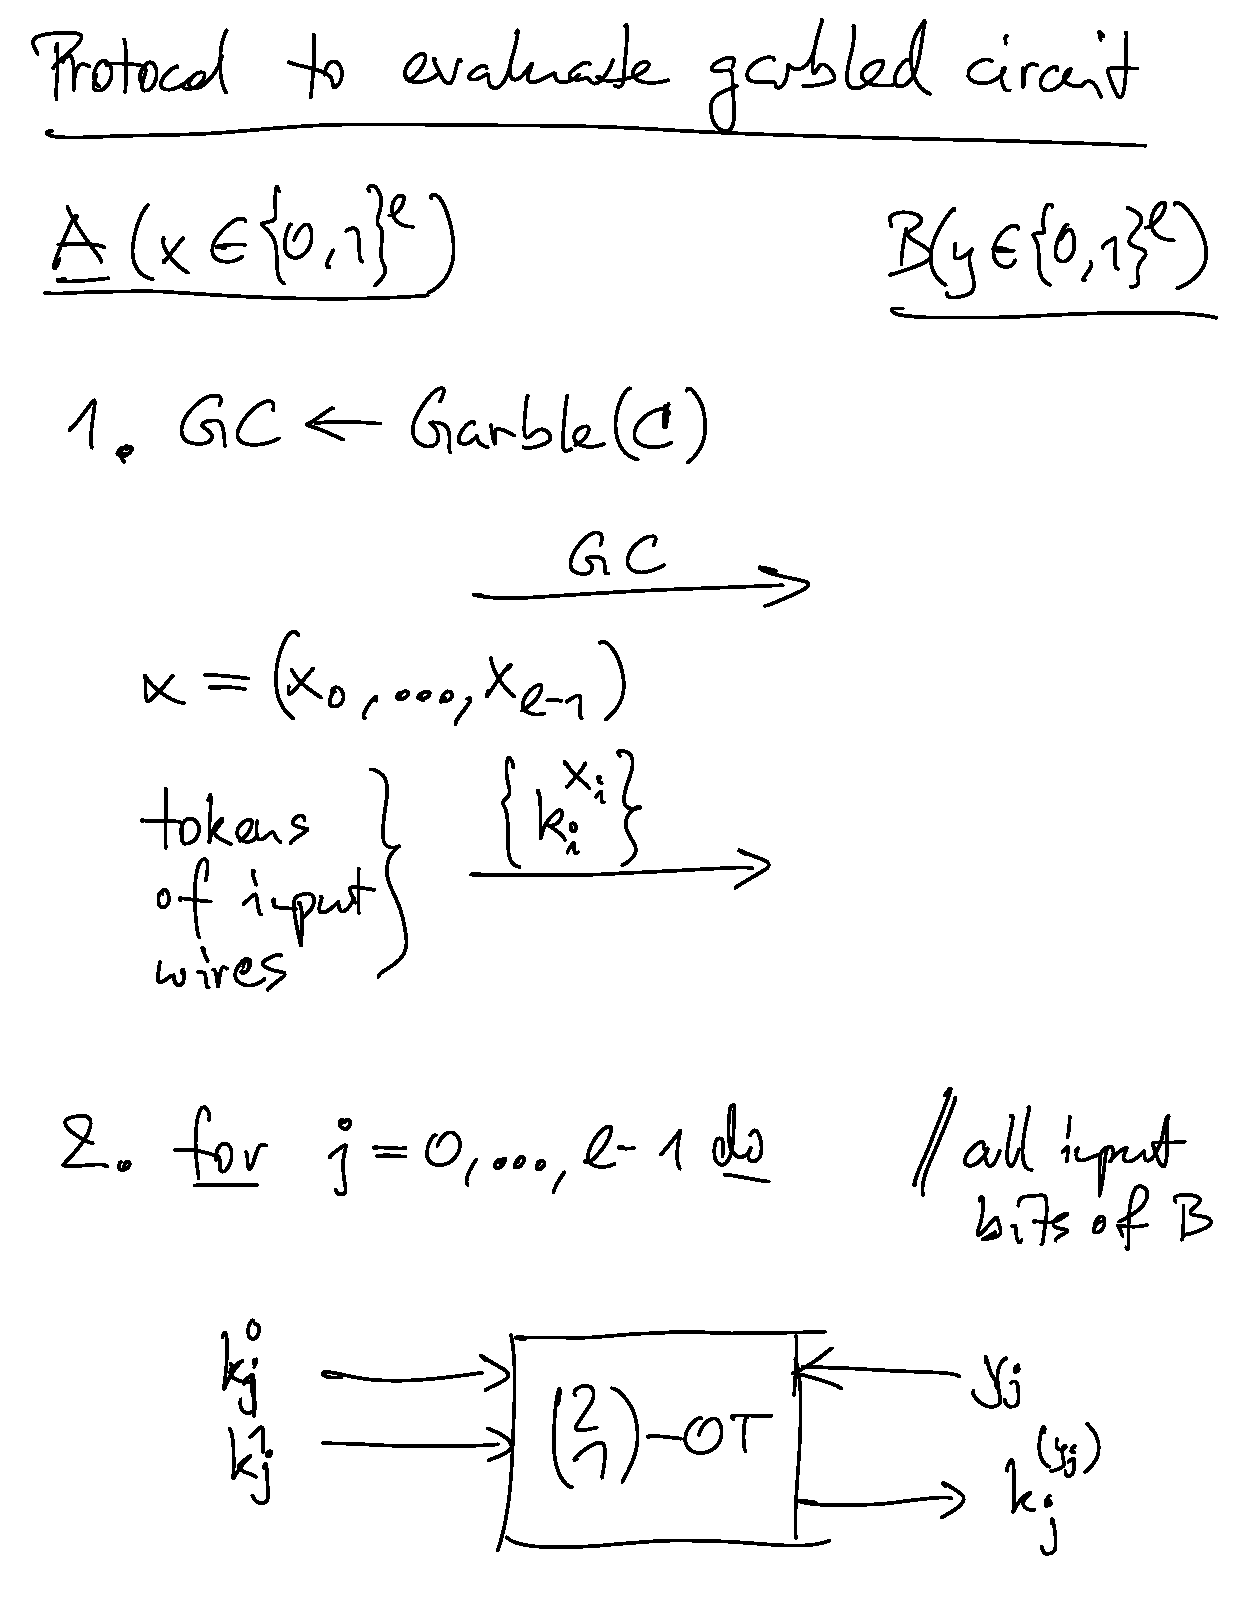
\includegraphics[width=0.7\textwidth]{8_evaluate}

Finally evaluate the garbled circuit, decode the output bits, and output value
$z = f(x, y)$.
